\documentclass[dvisvgm,border=2pt]{standalone}
% Shared by every figure. Two colours only: black becomes the text colour of
% whatever theme the app is in, and `accent` becomes the brand — see
% scripts/build-figures.mjs. Everything else is done with opacity.
\usepackage{amsmath}
\usepackage{amssymb}
\usepackage{tikz}
\usepackage{pgfplots}
\pgfplotsset{compat=1.18}
\usetikzlibrary{arrows.meta,positioning,calc,backgrounds,fit,patterns.meta}
\definecolor{accent}{RGB}{255,0,255}
\pgfplotsset{
  every axis/.append style={
    axis lines=left,
    axis line style={draw opacity=0.35},
    tick style={draw opacity=0.35},
    tick label style={font=\scriptsize,opacity=0.7},
    label style={font=\scriptsize,opacity=0.7},
    legend style={draw=none,fill=none,font=\scriptsize},
    every axis plot/.append style={line width=0.7pt},
  },
}
\tikzset{
  every picture/.style={font=\scriptsize},
  faint/.style={opacity=0.3},
  quiet/.style={opacity=0.55},
  box/.style={draw,opacity=0.35,rounded corners=2pt,inner sep=4pt},
  hot/.style={accent},
}

\begin{document}
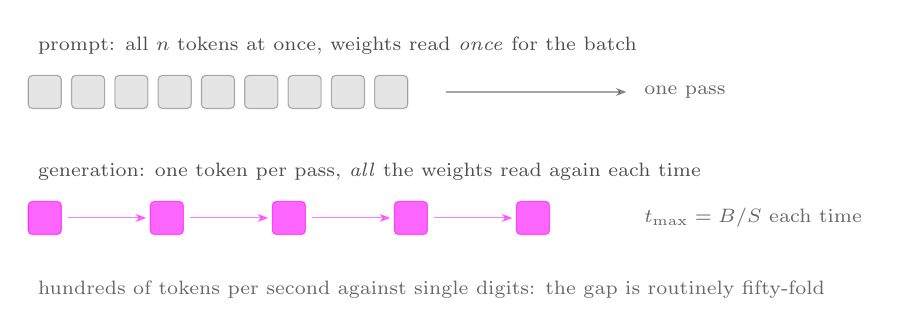
\begin{tikzpicture}[every node/.style={font=\scriptsize},x=1cm,y=1cm]
  \node[anchor=west,opacity=0.7] at (0,2.5) {prompt: all $n$ tokens at once, weights read \emph{once} for the batch};
  \foreach \i in {0,...,8}
    \draw[opacity=0.3,fill,fill opacity=0.1,rounded corners=1.5pt] (\i*0.55,1.7) rectangle ++(0.42,0.42);
  \draw[opacity=0.35,-{Stealth[length=4pt]}] (5.3,1.91) -- (7.6,1.91);
  \node[anchor=west,opacity=0.6] at (7.7,1.91) {one pass};
  \node[anchor=west,opacity=0.7] at (0,0.9) {generation: one token per pass, \emph{all} the weights read again each time};
  \foreach \i in {0,...,4}{
    \pgfmathsetmacro{\op}{0.25+\i*0.15}
    \draw[accent,fill=accent,fill opacity=\op,opacity=0.6,rounded corners=1.5pt]
      (\i*1.55,0.1) rectangle ++(0.42,0.42);
    \ifnum\i<4
      \draw[accent,opacity=0.5,-{Stealth[length=4pt]}] (\i*1.55+0.5,0.31) -- (\i*1.55+1.5,0.31);
    \fi
  }
  \node[anchor=west,opacity=0.6] at (7.7,0.31) {$t_{\max}=B/S$ each time};
  \node[anchor=west,opacity=0.6] at (0,-0.6) {hundreds of tokens per second against single digits: the gap is routinely fifty-fold};
\end{tikzpicture}
\end{document}
